% ESD protection in the IHP SG13CMOS5L I/O library -- working notes
% Compiled 2026-10-02 for sg13cmos5l_cm_ip__single2diff2single (Chipalooza 2026)
\documentclass[11pt,a4paper]{article}

\usepackage[utf8]{inputenc}
\usepackage[a4paper,margin=24mm]{geometry}
\usepackage[expansion=false]{microtype}
\usepackage{amsmath}
\usepackage{booktabs,tabularx,array}
\usepackage{siunitx}
\usepackage[europeanresistors,americaninductors]{circuitikz}
\usepackage{xcolor}
\usepackage{enumitem}
\usepackage[hidelinks]{hyperref}
\usepackage{xurl}

\setlist{itemsep=2pt,topsep=4pt}
\newcommand{\cell}[1]{\texttt{#1}}
\newcolumntype{L}{>{\raggedright\arraybackslash}X}
\sisetup{range-phrase=--}
\setlength{\emergencystretch}{3em}

\title{ESD Protection in the IHP SG13CMOS5L I/O Library\\[2pt]
  \large Structures, test methods, and literature --- notes for\\
  \texttt{sg13cmos5l\_cm\_ip\_\_single2diff2single} (Chipalooza 2026)}
\author{}
\date{2 October 2026}

\begin{document}
\maketitle

\begin{abstract}
\noindent
These notes summarise the electrostatic-discharge (ESD) protection used in the
open-source IHP \cell{sg13cmos5l\_io} pad library, as read from the CDL netlist
and measured in the GDS layout, and explain the background needed to discuss
resized clamp transistors with IHP (IHP-Open-PDK issue \#1252): the HBM, CDM and
TLP test methods, and the grounded-gate NMOS and its relatives. A short
annotated bibliography closes the document. Statements marked \emph{(inference)}
are inferences from the data, not documented by IHP.
\end{abstract}

\section{Summary}

The IHP I/O library uses a conventional, unexotic protection scheme:
\begin{itemize}
  \item \textbf{Primary pad-to-rail diodes} (\cell{DCNDiode} to iovss,
        \cell{DCPDiode} to iovdd) on every signal pad.
  \item An \textbf{RC-triggered rail clamp} (a \SI{757}{\micro\metre}-wide
        thick-oxide NMOS) in every supply pad.
  \item \textbf{Large multi-finger thick-oxide MOSFETs on the pad}: on output
        pads these are the drivers themselves; on the analog pad they are the
        same transistor arrays with the gate tied off through a resistor.
  \item A \textbf{secondary stage} (series resistor plus small diodes) in front
        of anything with a gate connected to the pad.
\end{itemize}
There are no SCRs, no silicide-block drain ballasting, and the I/O cells do not
carry the ESD recognition layer (\cell{Recog.esd}, 99/30).

\paragraph{Origin of the cells.}
The README of the sibling \cell{sg13g2\_io} library states that the cells were
generated by the Chips4Makers Python flow (repository
\cell{c4m-pdk-ihpsg13g2}, Staf Verhaegen), version 0.0.4, and later patched by
IHP (``I/O Update 2'', 18 June 2026, which among other things notes
``Analog Pad current capability is improved'', issue \#401). The
\cell{sg13cmos5l\_io} cells have the identical structure. The clamp cells
were therefore originally the output of a parametric generator, and Chips4Makers
is a second possible point of contact on design intent.

\section{Building blocks}

Table~\ref{tab:blocks} lists the protection subcircuits in
\cell{sg13cmos5l\_io.cdl}; Figures~\ref{fig:analog} and~\ref{fig:railclamp}
show the analog pad and the rail clamp.

\begin{table}[htb]
\centering\small
\caption{ESD building blocks in \cell{sg13cmos5l\_io}.}
\label{tab:blocks}
\begin{tabularx}{\linewidth}{@{}>{\raggedright\arraybackslash}p{0.25\linewidth}L>{\raggedright\arraybackslash}p{0.2\linewidth}@{}}
\toprule
Cell & What it is & Used in\\
\midrule
\cell{DCNDiode}, \cell{DCPDiode} &
  Primary diodes: n+/p-sub (\cell{dantenna}) from iovss to pad, p+/n-well
  (\cell{dpantenna}) from pad to iovdd. Each is two
  \SI{1.26}{\micro\metre}\,$\times$\,\SI{27.78}{\micro\metre} stripes. &
  every signal pad; supply-ground pads\\
\addlinespace
\cell{Clamp\_N43N43D4R},\newline \cell{RCClampResistor},\newline \cell{RCClampInverter} &
  Rail clamp: 172 fingers of \SI{4.4}{\micro\metre}/\SI{0.6}{\micro\metre}
  \cell{sg13\_hv\_nmos} (\SI{757}{\micro\metre} total). Trigger:
  $26\times\SI{5.24}{\kilo\ohm}$ rppd (\SI{136}{\kilo\ohm}) into a
  $\approx$\SI{1200}{\micro\metre\squared} thick-oxide MOS capacitor;
  inverter (PMOS \SI{350}{\micro\metre}/\SI{0.5}{\micro\metre},
  NMOS $2\times\SI{54}{\micro\metre}$/\SI{0.5}{\micro\metre}) drives the gate. &
  \cell{IOPadVdd}, \cell{IOPadIOVdd}\\
\addlinespace
\cell{Clamp\_\{N,P\}}\allowbreak\cell{\{2,8,15\}N\ldots D} &
  Output drivers that double as the ESD device; gate is a pin, driven by
  \cell{GateLevelUpInv}. &
  \cell{IOPadOut}, \cell{TriOut}, \cell{InOut} (4/16/30\,mA)\\
\addlinespace
\cell{Clamp\_N20N0D}, \cell{Clamp\_P20N0D} &
  Same arrays with gate tied off through rppd: \SI{1.96}{\kilo\ohm} to iovss
  (gate-coupled NMOS) and \SI{6.77}{\kilo\ohm} to iovdd (gate-to-VDD PMOS). &
  \cell{IOPadAnalog} only\\
\addlinespace
\cell{SecondaryProtection} &
  \SI{587}{\ohm} rppd series resistor plus small \cell{dantenna}/\cell{dpantenna}
  diodes to the rails. &
  \cell{IOPadAnalog} (\cell{padres}), \cell{LevelDown}\\
\bottomrule
\end{tabularx}
\end{table}

\begin{figure}[htb]
\centering
\begin{circuitikz}[scale=0.76, transform shape, line width=0.6pt]
  % rails
  \draw (0,6) node[left]{iovdd} -- (15.6,6);
  \draw (0,0) node[left]{iovss} -- (15.6,0);
  % pad and pad bus
  \draw (0,3) node[draw, fill=gray!20, minimum width=11mm, minimum height=8mm, anchor=east]{PAD} -- (8.3,3);
  % primary diodes
  \draw (1.5,3) to[D*, l_={DCP}, *-*] (1.5,6);
  \draw (1.5,0) to[D*, l_={DCN}, *-] (1.5,3);
  % GDPMOS  Clamp_P20N0D
  \node[pmos, anchor=D] (mp) at (5.2,3) {};
  \draw (mp.S) -- (mp.S |- 0,6) node[circ]{};
  \draw (mp.D) node[circ]{};
  \draw (mp.G) -- ++(-0.9,0) coordinate (gp) to[R, l_={\SI{6.77}{\kilo\ohm}}] (gp |- 0,6) node[circ]{};
  \node[anchor=west, font=\footnotesize] at ($(mp.S)+(0.25,-0.55)$) {\cell{Clamp\_P20N0D}};
  % GCNMOS  Clamp_N20N0D
  \node[nmos, anchor=D] (mn) at (5.2,3) {};
  \draw (mn.S) -- (mn.S |- 0,0) node[circ]{};
  \draw (mn.G) -- ++(-0.9,0) coordinate (gn) to[R, l={\SI{1.96}{\kilo\ohm}}] (gn |- 0,0) node[circ]{};
  \node[anchor=west, font=\footnotesize] at ($(mn.S)+(0.25,0.55)$) {\cell{Clamp\_N20N0D}};
  % secondary protection
  \draw (8.3,3) to[R, l={\SI{587}{\ohm}}] (10.8,3) node[circ]{};
  \draw (10.8,0) node[circ]{} to[D*, l_={\cell{dantenna}}] (10.8,3);
  \draw (10.8,3) to[D*, l_={\cell{dpantenna}}] (10.8,6) node[circ]{};
  \draw (10.8,3) -- (12.6,3) node[right]{\cell{padres}};
  \draw[dashed, gray] (7.9,0.35) rectangle (12.4,5.65);
  \node[gray, font=\scriptsize, anchor=north west] at (7.95,5.6) {\cell{SecondaryProtection}};
  % rail clamp (lives in the supply pads)
  \draw (14.9,0) node[circ]{} to[generic, l_={rail clamp (Fig.~\ref{fig:railclamp})}] (14.9,6) node[circ]{};
\end{circuitikz}
\caption{ESD network of \cell{sg13cmos5l\_IOPadAnalog} (from the CDL). The core
connects to \cell{padres}, behind the \SI{587}{\ohm} secondary resistor. NMOS
bulk is the substrate (tied to iovss through ptap guard rings), PMOS bulk is
iovdd. The rail clamp is not part of this pad; it sits in the
\cell{IOPadVdd}/\cell{IOPadIOVdd} supply pads and completes the
pad\,$\to$\,iovdd\,$\to$\,iovss discharge path.}
\label{fig:analog}
\end{figure}

\begin{figure}[htb]
\centering
\begin{circuitikz}[scale=0.85, transform shape, line width=0.6pt]
  \draw (0,4.5) node[left]{iovdd / vdd} -- (9.5,4.5);
  \draw (0,0) node[left]{iovss} -- (9.5,0);
  \draw (1.5,4.5) node[circ]{} to[R, l_={\SI{136}{\kilo\ohm}}, -*] (1.5,2.25) coordinate (n1);
  \draw (n1) to[C, l_={MOS cap $\approx\SI{1200}{\micro\metre\squared}$}] (1.5,0) node[circ]{};
  \node[not port] (inv) at (4.6,2.25) {};
  \draw (n1) -- (inv.in);
  \node[font=\footnotesize, below] at (inv.south) {\cell{RCClampInverter}};
  \node[nmos] (mc) at (7.6,2.25) {};
  \draw (inv.out) -- (mc.G);
  \draw (mc.D) -- (mc.D |- 0,4.5) node[circ]{};
  \draw (mc.S) -- (mc.S |- 0,0) node[circ]{};
  \node[anchor=west, font=\footnotesize, align=left] at ($(mc.D)+(0.3,-0.6)$)
    {\cell{Clamp\_N43N43D4R}\\$172\times\SI{4.4}{\micro\metre}/\SI{0.6}{\micro\metre}$};
\end{circuitikz}
\caption{RC-triggered rail clamp in \cell{IOPadVdd} and \cell{IOPadIOVdd}
(inverter supplied from the protected rail and iovss). On a fast ESD edge the
capacitor holds the inverter input low, the inverter drives the clamp gate
high, and the clamp conducts through its channel --- no snapback is involved.
On a slow power-up the input follows the rail and the clamp stays off. With a
thick-oxide $C_\mathrm{ox}$ of roughly \SI{5}{\femto\farad\per\micro\metre\squared}
the time constant is on the order of \SI{1}{\micro\second} \emph{(inference;
$C_\mathrm{ox}$ not taken from IHP data)}.}
\label{fig:railclamp}
\end{figure}

\begin{table}[htb]
\centering\small
\caption{Which protection device sits on which pad (from \cell{sg13cmos5l\_io.cdl}).}
\label{tab:pads}
\begin{tabularx}{\linewidth}{@{}lLLL@{}}
\toprule
Pad & Pad $\to$ iovss & Pad $\to$ iovdd & Other\\
\midrule
\cell{IOPad\{Out,TriOut,InOut\}4mA}  & \cell{Clamp\_N2N2D} (driver)   & \cell{Clamp\_P2N2D} (driver)   & DCN/DCP diodes\\
\cell{IOPad\{Out,TriOut,InOut\}16mA} & \cell{Clamp\_N8N8D} (driver)   & \cell{Clamp\_P8N8D} (driver)   & DCN/DCP diodes\\
\cell{IOPad\{Out,TriOut,InOut\}30mA} & \cell{Clamp\_N15N15D} (driver) & \cell{Clamp\_P15N15D} (driver) & DCN/DCP diodes\\
\cell{IOPadAnalog} & \cell{Clamp\_N20N0D} (GCNMOS) & \cell{Clamp\_P20N0D} (GDPMOS) & diodes, secondary stage\\
\cell{IOPadIn}     & --- & --- & diodes; secondary stage inside \cell{LevelDown}\\
\cell{IOPadVdd}, \cell{IOPadIOVdd} & \multicolumn{2}{l}{\cell{Clamp\_N43N43D4R}, RC-triggered rail clamp} & \\
\cell{IOPadVss}, \cell{IOPadIOVss} & \multicolumn{2}{l}{---} & DCN/DCP diodes\\
\bottomrule
\end{tabularx}
\end{table}

Table~\ref{tab:pads} shows which device sits on which pad. All pad clamps use the same finger cell; only the gate connection differs.
The analog pad's 20-finger pair is larger than even the 30\,mA driver.

\section{Clamp geometry (measured from the GDS)}

The following was measured with the KLayout Python API on
\cell{sg13cmos5l\_io.gds} from the IHP-Open-PDK \cell{dev} branch.
\begin{itemize}
  \item Devices: \cell{sg13\_hv\_nmos} and \cell{sg13\_hv\_pmos}, $L=\SI{0.6}{\micro\metre}$.
        Finger width \SI{4.4}{\micro\metre} (NMOS) and \SI{6.66}{\micro\metre} (PMOS).
        PMOS cells contain two rows, so \cell{P20} has 40 gates.
  \item Finger pitch alternates \SI{1.78}{\micro\metre} / \SI{1.24}{\micro\metre}.
        Contact-to-gate spacing is \SI{0.51}{\micro\metre} on the shared drains
        (confirmed by net tracing: the wide strips connect to \cell{pad}) and
        \SI{0.24}{\micro\metre} on the shared sources (\cell{iovss}/\cell{iovdd}).
        This extra drain spacing is the only ballasting.
  \item Drains are fully silicided: \cell{SalBlock} appears only on the rppd
        gate resistors of the \cell{N0D} variants.
  \item No \cell{Recog.esd} (99/30) layer: the clamps extract and pass LVS as
        ordinary HV MOSFETs. Each cell has its own ptap guard ring.
  \item Cell width \SIrange{80.4}{81.2}{\micro\metre}, matching the pad pitch.
  \item Naming \emph{(inference)}: \cell{Clamp\_\{N,P\}$a$N$b$D[$r$R]} reads as
        $a$ fingers per row, $b$ of them with a driven gate ($b=0$: gate tied
        off), and $r$ rows (\cell{4R}: $43\times4=172$ fingers).
\end{itemize}

\section{Standalone ESD devices in \cell{SG13\_dev}}

The PCell \cell{esd\_code.py} offers \cell{diodevdd\_2kv}, \cell{diodevdd\_4kv},
\cell{diodevss\_2kv}, \cell{diodevss\_4kv}, \cell{nmoscl\_2} and \cell{nmoscl\_4}.
They are fixed layouts (the only parameter is the model name), drawn with
\cell{Recog.esd} plus a text label, which the DRC deck uses to exempt them from
antenna, well-crossing and salicide-block-resistor rules. They are the only
place in the open PDK that states a kV rating. The I/O library does not use
them. The DRC deck also recognises an \cell{scr1} device, for which CMOS5L ships
no PCell.

\section{ESD test methods: HBM, CDM and TLP}

\paragraph{HBM (Human Body Model).}
Models a charged person touching a pin: a \SI{100}{\pico\farad} capacitor
charged to the test voltage and discharged into the pin through
\SI{1.5}{\kilo\ohm}, giving a pulse with a rise time of a few nanoseconds and a
decay time constant of about \SI{150}{\nano\second}. Peak current is
approximately $V/\SI{1.5}{\kilo\ohm}$, so \SI{2}{\kilo\volt} HBM corresponds to
about \SI{1.3}{\ampere}. Standardised in ANSI/ESDA/JEDEC JS-001; performed on
packaged parts over pin combinations, with a pass/fail voltage as the result.

\paragraph{CDM (Charged Device Model).}
The device itself is charged and discharges through a single pin: a pulse of
about \SI{1}{\nano\second} with several amperes peak. Standardised in
ANSI/ESDA/JEDEC JS-002. CDM is the threat a secondary stage such as
\cell{SecondaryProtection} primarily addresses, since the charge resides on the
die and stresses the thin input gates directly.

\paragraph{TLP (Transmission Line Pulse).}
A characterisation method, not a qualification test. A charged length of
coaxial line is discharged into the device under test, producing a clean
rectangular pulse, typically \SI{100}{\nano\second} wide, comparable in energy
to an HBM event. The amplitude is stepped; at each step voltage and current
are averaged over the flat part of the pulse, and a DC leakage measurement
after each pulse detects damage. The result is the I--V curve in the ESD
regime (Fig.~\ref{fig:tlp}). Standardised in ANSI/ESD STM5.5.1; the
\SIrange{1}{5}{\nano\second} variant (vf-TLP) correlates with CDM.

\begin{figure}[htb]
\centering
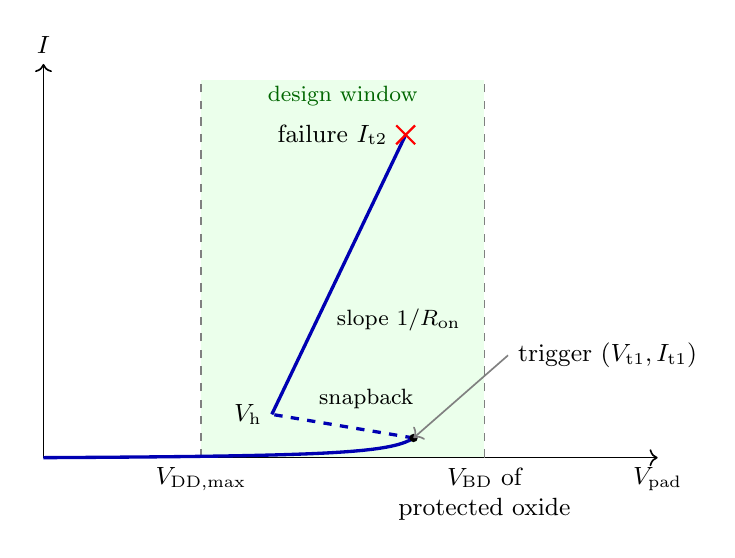
\begin{tikzpicture}[scale=1.0, line width=0.6pt, font=\small]
  % design window
  \fill[green!8] (2.0,0) rectangle (5.6,4.8);
  \node[green!40!black, font=\footnotesize] at (3.8,4.6) {design window};
  % axes
  \draw[->] (0,0) -- (7.8,0) node[below]{$V_\mathrm{pad}$};
  \draw[->] (0,0) -- (0,5) node[above]{$I$};
  % limits
  \draw[dashed, gray] (2.0,0) node[below, black]{$V_\mathrm{DD,max}$} -- (2.0,4.8);
  \draw[dashed, gray] (5.6,0) node[below, black, align=center]{$V_\mathrm{BD}$ of\\protected oxide} -- (5.6,4.8);
  % curve
  \draw[very thick, blue!70!black] (0,0) .. controls (3.5,0.02) and (4.4,0.05) .. (4.7,0.25) coordinate (t1);
  \draw[very thick, blue!70!black, dashed] (t1) -- (2.9,0.55) coordinate (h);
  \draw[very thick, blue!70!black] (h) -- (4.6,4.1) coordinate (t2);
  \draw[red, thick] (t2) ++(-0.12,-0.12) -- ++(0.24,0.24) ++(0,-0.24) -- ++(-0.24,0.24);
  % annotations
  \fill (t1) circle (1.5pt); \draw[<-, gray] (t1) -- (5.9,1.3) node[right, black]{trigger $(V_\mathrm{t1}, I_\mathrm{t1})$};
  
  \node[left] at (h) {$V_\mathrm{h}$};
  \node[left, xshift=-3pt] at (t2) {failure $I_\mathrm{t2}$};
  \node[right, font=\footnotesize] at (3.6,1.75) {slope $1/R_\mathrm{on}$};
  \node[font=\footnotesize] at (4.1,0.75) {snapback};
\end{tikzpicture}
\caption{Qualitative TLP I--V curve of a snapback device (GGNMOS); illustrative,
not IHP data. $V_\mathrm{t1}$ must lie inside the design window; $V_\mathrm{h}$
below $V_\mathrm{DD,max}$ risks a latched-on clamp in normal operation;
$I_\mathrm{t2}$ sets the robustness, with the rule of thumb
HBM rating $\approx I_\mathrm{t2}\times\SI{1.5}{\kilo\ohm}$.}
\label{fig:tlp}
\end{figure}

\paragraph{Why it matters here.}
$I_\mathrm{t2}$ is normally quoted per micrometre of gate width for a given
finger design (L, drain contact-to-gate spacing, silicidation). With TLP data
for IHP's \SI{4.4}{\micro\metre}/\SI{0.6}{\micro\metre} finger, choosing a finger
count is arithmetic, subject to uniform triggering of all fingers. Changing the
finger geometry itself invalidates any per-micrometre figure. The most specific
question to put to IHP is therefore whether TLP curves exist for the
\cell{Clamp\_*} finger cells.

\section{GGNMOS and related devices}

\begin{figure}[htb]
\centering
\begin{circuitikz}[scale=0.9, transform shape, line width=0.6pt, font=\small]
  % substrate
  \draw (0,0) rectangle (10,3);
  \node[anchor=south west, font=\footnotesize] at (0.1,0.05) {p-substrate};
  % diffusions
  \draw[fill=blue!12] (1.5,2.4) rectangle (3.5,3); \node at (2.5,2.7) {n+};
  \draw[fill=blue!12] (5.0,2.4) rectangle (7.0,3); \node at (6.0,2.7) {n+};
  \draw[fill=red!12]  (8.2,2.4) rectangle (9.5,3); \node at (8.85,2.7) {p+};
  % gate
  \draw[fill=gray!35] (3.5,3.05) rectangle (5.0,3.45); \node[font=\footnotesize] at (4.25,3.25) {gate};
  % terminals
  \draw (2.5,3) -- (2.5,3.9) node[above]{pad (drain)};
  \draw (4.25,3.45) -- (4.25,4.5) node[above]{VSS (or $R_g$ to VSS)};
  \draw (6.0,3) -- (6.0,3.9) node[above]{VSS (source)};
  \draw (8.85,3) -- (8.85,3.9) node[above]{VSS (tap)};
  % parasitic npn
  \node[npn, rotate=90] (q) at (4.25,1.35) {};
  \draw (q.C) -| (2.5,2.4);
  \draw (q.E) -| (6.0,2.4);
  \draw (q.B) -- (q.B |- 0,0.5) -- (8.85,0.5) to[R, l_={$R_\mathrm{sub}$}] (8.85,2.4);
  \node[font=\footnotesize, red!60!black, align=center] at (1.0,1.7) {avalanche\\at drain\\junction};
\end{circuitikz}
\caption{Cross-section of a grounded-gate NMOS with its parasitic lateral NPN
(collector = drain, base = substrate, emitter = source) and the substrate
resistance $R_\mathrm{sub}$ to the ptap.}
\label{fig:ggnmos}
\end{figure}

\paragraph{GGNMOS (grounded-gate NMOS).}
Drain to the pad; gate, source and bulk to VSS. The device is off in normal
operation and protects through its parasitic lateral NPN (Fig.~\ref{fig:ggnmos}).
On a positive zap the drain--substrate junction avalanches at $V_\mathrm{t1}$;
avalanche holes flowing through $R_\mathrm{sub}$ to the ptap raise the local
substrate potential until the source junction forward-biases; the NPN turns on
and the voltage snaps back to $V_\mathrm{h}$, after which the device carries
amperes until it fails at $I_\mathrm{t2}$. On a negative zap the
drain--substrate diode simply conducts forward. The known weakness is
multi-finger triggering: the first finger to snap back pulls the pad below the
others' $V_\mathrm{t1}$, and if $V_\mathrm{t2}<V_\mathrm{t1}$ that single finger
carries all the current and fails. Remedies are drain ballast resistance
(silicide block, larger drain contact spacing) and gate coupling.

\paragraph{GCNMOS (gate-coupled NMOS).}
The gate is tied to VSS through a resistor rather than directly. The fast ESD
edge couples onto the gate through the gate--drain overlap capacitance; the
channel conducts briefly, which lowers $V_\mathrm{t1}$ and makes the fingers
trigger together. IHP's \cell{Clamp\_N20N0D} (\SI{1.96}{\kilo\ohm} to iovss) is
of this kind.

\paragraph{GDPMOS (gate-to-VDD PMOS).}
The mirror image: drain to pad; source, gate and n-well to VDD. The parasitic
PNP snaps back weakly or not at all in modern processes, so the device mainly
acts as a p+/n-well diode from pad to VDD plus a breakdown path. IHP's
\cell{Clamp\_P20N0D} (\SI{6.77}{\kilo\ohm} to iovdd) is of this kind.

\paragraph{Self-protecting output driver.}
An output NMOS/PMOS large enough to serve as its own clamp. During an ESD event
on an unpowered chip the pre-driver does not actively drive the gates, so the
drivers behave roughly like GGNMOS/GDPMOS. All IHP output pads use this scheme.

\paragraph{RC-triggered (active) rail clamp.}
A large MOSFET that conducts through its channel, with the gate driven by an RC
transient detector; no snapback is required (Fig.~\ref{fig:railclamp}).

\paragraph{SCR / LVTSCR.}
Thyristor-based clamps: very area-efficient but latch-up-prone. Not used in the
IHP I/O library.

\section{Implications for resized clamp PCells}

\begin{itemize}
  \item \textbf{DRC and LVS do not check ESD robustness.} The only ESD-related
        checks in the CMOS5L layout rules are the latch-up rules LU.a--LU.d
        (\S7.2, off by default), together with guidelines for output buffers:
        guard rings around every pad-connected device, and double guard rings
        between N and P drivers and between drivers and core. Enabling the LU
        check is worthwhile.
  \item \textbf{Conservative path:} keep the finger cell identical (L, W, drain
        spacing, contact pattern, guard ring) and change only the finger
        count. Robustness then scales roughly with total width, provided all
        fingers trigger uniformly; with silicided drains, uniform triggering is
        the weak point, which is what the gate-coupling resistors of the
        \cell{N0D} variants address.
  \item \textbf{Argument for IHP:} an output driver at least as wide as
        \cell{N8N8D}/\cell{P8N8D}, alongside the DCN/DCP diodes, is structurally
        the same as IHP's own 16\,mA output pad.
  \item \textbf{What only IHP can supply:} TLP/HBM data for these cells. No ESD
        rating for the I/O library was found in the open PDK.
\end{itemize}

\section{Observed netlist defect}

In \cell{sg13cmos5l\_IOPadInOut30mA} the instance
\begin{center}
\cell{XI3 net2 iovss pad ptap1 / sg13cmos5l\_Clamp\_N15N15D}
\end{center}
passes four nodes to a three-port subcircuit. A SPICE simulator should reject
this; it may merit a separate one-line issue.

\section{Literature}

\subsection*{Books}
\begin{enumerate}[label={[B\arabic*]}, leftmargin=*]
  \item A.~Amerasekera and C.~Duvvury, \emph{ESD in Silicon Integrated
        Circuits}, 2nd ed. Wiley, 2002. --- The standard reference on device
        physics (snapback, second breakdown, silicide effects) and protection
        design.
  \item S.~Dabral and T.~J.~Maloney, \emph{Basic ESD and I/O Design}. Wiley,
        1998. --- Written from the I/O designer's perspective; closest in
        spirit to the pad work here.
  \item S.~H.~Voldman, \emph{ESD: Physics and Devices}, Wiley, 2004; and
        \emph{ESD: Circuits and Devices}, Wiley, 2006 (2nd ed.\ 2015). ---
        Broad series; the circuits volume covers rail clamps and I/O networks.
  \item A.~Z.~H.~Wang, \emph{On-Chip ESD Protection for Integrated Circuits:
        An IC Design Perspective}. Kluwer, 2002.
  \item O.~Semenov, H.~Sarbishaei and M.~Sachdev, \emph{ESD Protection Device
        and Circuit Design for Advanced CMOS Technologies}. Springer, 2008. ---
        Has dedicated chapters on circuit concepts and on power (rail) clamps.
\end{enumerate}

\subsection*{Foundational papers}
\begin{enumerate}[label={[P\arabic*]}, leftmargin=*]
  \item T.~J.~Maloney and N.~Khurana, ``Transmission line pulsing techniques
        for circuit modeling of ESD phenomena,'' \emph{Proc.\ EOS/ESD Symp.},
        EOS-7, pp.~49--54, 1985. --- Origin of TLP.
  \item C.~H.~Polgreen and A.~Chatterjee, ``Improving the ESD failure threshold
        of silicided n-MOS output transistors by ensuring uniform current
        flow,'' \emph{IEEE Trans.\ Electron Devices}, vol.~39, no.~2, 1992.
        \emph{(volume/issue not independently verified)} --- Directly addresses
        the multi-finger uniformity problem of silicided drivers like IHP's.
  \item R.~Merrill and E.~Issaq, ``ESD design methodology,'' \emph{Proc.\
        EOS/ESD Symp.}, EOS-15, pp.~233--237, 1993. --- Early statement of the
        rail-based (diodes plus power clamp) protection scheme.
  \item E.~R.~Worley \emph{et al.}, ``Sub-micron chip ESD protection schemes
        which avoid avalanching junctions,'' \emph{Proc.\ EOS/ESD Symp.},
        EOS-17, pp.~13--20, 1995. --- The RC-triggered MOSFET rail clamp.
  \item J.~Z.~Chen, E.~A.~Amerasekera and C.~Duvvury, ``Design methodology and
        optimization of gate-driven NMOS ESD protection circuits in submicron
        CMOS processes,'' \emph{IEEE Trans.\ Electron Devices}, vol.~45, no.~12,
        pp.~2448--2456, 1998, doi:10.1109/16.735721. --- Gate coupling
        (GCNMOS) for uniform multi-finger turn-on.
  \item M.-D.~Ker, ``Whole-chip ESD protection design with efficient
        VDD-to-VSS ESD clamp circuits for submicron CMOS VLSI,'' \emph{IEEE
        Trans.\ Electron Devices}, vol.~46, no.~1, pp.~173--183, 1999.
\end{enumerate}

\subsection*{Freely available}
\begin{enumerate}[label={[F\arabic*]}, leftmargin=*]
  \item J.-H.~Chun, \emph{ESD Protection Circuits for Advanced CMOS
        Technologies}, Ph.D.\ dissertation, Stanford University, 2006.
        \url{http://www-tcad.stanford.edu/tcad/pubs/theses/chun.pdf}
  \item Industry Council on ESD Target Levels, \emph{White Paper 1: A Case for
        Lowering Component Level HBM/MM ESD Specifications and Requirements},
        and \emph{White Paper 2: A Case for Lowering Component Level CDM ESD
        Specifications and Requirements} (Rev.~3.0, 2021).
        \url{https://www.esdindustrycouncil.org/ic/en/documents} --- Why
        \SI{1}{\kilo\volt} HBM / \SI{250}{\volt} CDM-class targets are
        considered safe with basic factory ESD control.
  \item ESDA / In Compliance, ``Characterization for ESD Design, the TLP Zoo''
        (article series).
        \url{https://www.esda.org/news/characterization-for-esd-design-the-tlp-zoo-part-2/}
  \item ``Transmission Line Pulse Testing: The Indispensable Tool for ESD
        Characterization of Devices, Circuits and Systems,'' \emph{In
        Compliance Magazine}.
        \url{https://incompliancemag.com/transmission-line-pulse-testing-the-indispensable-tool-for-esd-characterization-of-devices-circuits-and-systems/}
  \item M.-D.~Ker's ESD reference list (NYCU).
        \url{https://alab.iee.nycu.edu.tw/~mdker/ESD/refer/refer.html}
\end{enumerate}

\subsection*{Standards}
ANSI/ESDA/JEDEC JS-001 (HBM); ANSI/ESDA/JEDEC JS-002 (CDM);
ANSI/ESD STM5.5.1 (TLP); ANSI/ESD SP5.5.2 (vf-TLP).

\subsection*{PDK sources used for Sections 1--7}
\begin{itemize}
  \item IHP-Open-PDK (\cell{dev} branch):
        \path{ihp-sg13cmos5l/libs.ref/sg13cmos5l_io/cdl/sg13cmos5l_io.cdl},
        \path{.../gds/sg13cmos5l_io.gds},
        \path{ihp-sg13g2/libs.ref/sg13g2_io/doc/README.md},
        \path{ihp-sg13cmos5l/libs.doc/doc/SG13CMOS5L_os_layout_rules.pdf} (\S7.2),
        \path{.../sg13cmos5l_pycell_lib/ihp/esd_code.py}.
        \url{https://github.com/IHP-GmbH/IHP-Open-PDK}
  \item IHP-Open-PDK issue \#1252.
        \url{https://github.com/IHP-GmbH/IHP-Open-PDK/issues/1252}
  \item Chips4Makers, \cell{c4m-pdk-ihpsg13g2}.
        \url{https://gitlab.com/Chips4Makers/c4m-pdk-ihpsg13g2}
\end{itemize}

\end{document}
